\documentclass[a4paper,10pt]{article}
\usepackage[utf8]{inputenc}
\usepackage{hyperref}
\usepackage{graphicx}
\DeclareGraphicsExtensions{.pdf}
\usepackage{fancyhdr}


\usepackage[top=1cm,bottom=1cm,left=2cm,right=2cm,includehead,head=2.5cm,headsep=0.499cm,includefoot,foot=12pt,footskip=2.8cm]{geometry}



% Pages styles
\fancypagestyle{Title}{\fancyhf{}
  \fancyhead[RO]{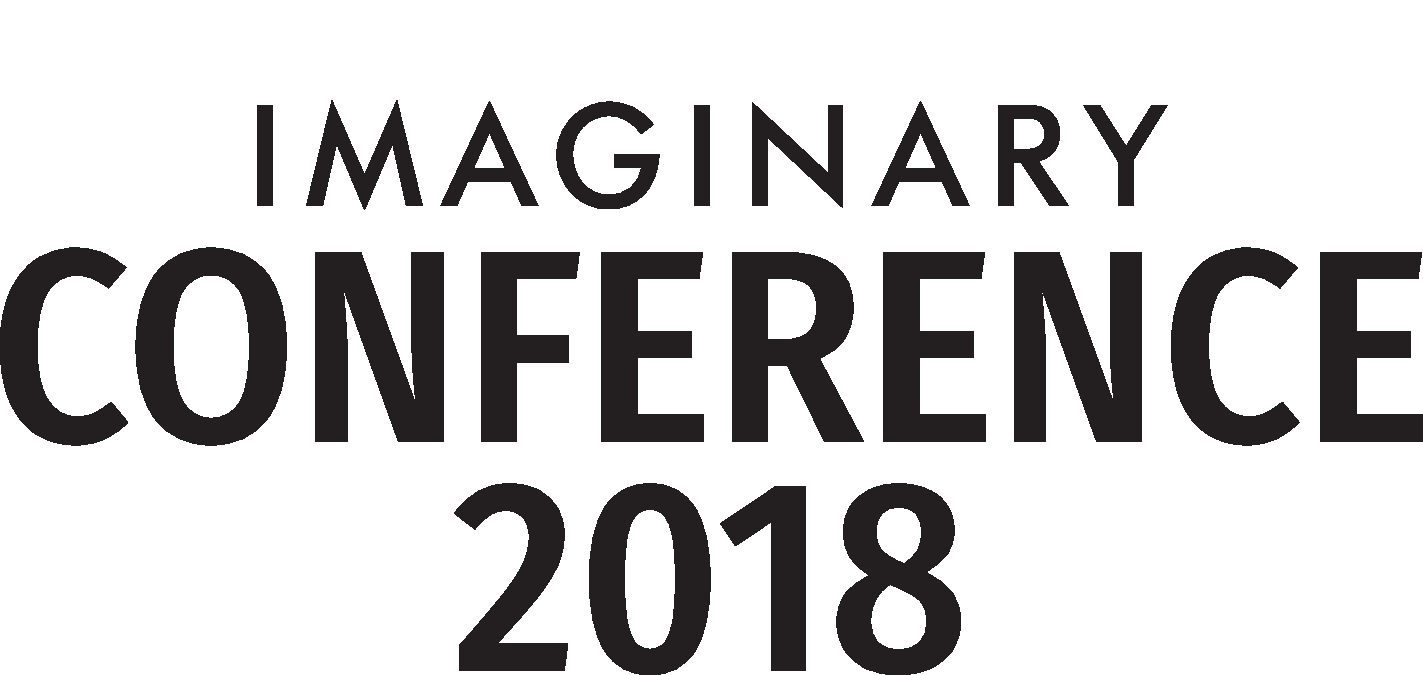
\includegraphics[width=5cm]{IC18-Logo-darkblue.pdf}}
 \renewcommand\headrulewidth{0pt}
}



% Title Page
\title{RPolyhedra: Experiences and beyond}
\author{Alejandro Baranek and Leonardo Belen}

\begin{document}

\maketitle
\thispagestyle{Title} 


\begin{abstract}
An R based library to explore and manipulate Polyhedra from different sources, with OpenGL rendering capabilities. Experiences compiling the library and taking it to the real life.  
\end{abstract}


\section{Information about the speakers}

\subsection{Personal Data}
BARANEK, Alejandro \\
Statistics Specialist \\
BELEN, Leonardo \\
Business Administration Specialist \\

\textbf{Address}: 2233 Rodriguez st., Buenos Aires, Argentina \\
\textbf{Tels.}: +54 (911) 6106-7032 / +54 (911) 6030 4529\\
\textbf{Web}: https://qbotics.shinyapps.io/rpolyhedra-explorer \\



\subsection{Speaker information for the conference program}

%Please add a short description of yourself for our conference program (max. 3 sentences). We appreciate to receive a low-resolution photo of you for the conference website. If you agree, please upload your photo as a separate file in the submission form.


Geometric lab is a project created by Alejandro Baranek and Leonardo Belen researching productivity techinques to close the gap bringing polyhedra to the physical world, for science, design, art and educational proposes.


Rpolyhedra is an R package published in CRAN and under review in RopenSci which compiles and distribute +800 polyhedra definitions from freely availables sources on the internet.


     

\section{Information about the talk}

\subsection{Talk classification}

%There is no restriction on the topics you can present. However, in case your talk fits within the five general conference topics (see \url{http://ic18.imaginary.org/ for details}), please select it below:
%\begin{itemize}
%\item Visualization, new tools and creation of mathematics exhibits
%\item Community, networking 
%\item Knowledge transfer and pedagogics 
%\item Mathematical writing, journalism and media
%\end{itemize}
\begin{itemize}
\item Visualization, new tools and creation of mathematics exhibits
\item Knowledge transfer and pedagogics 
\end{itemize}

\subsection{Talk overview: Fill the world with polyhedra}
%Describe here the content of your talk: State the main questions you address in your talk, describe the background of these questions and your main ideas. You can write max. 2 pages excluding references.

%Pictures with meaningful relation to your topic are welcome, but not mandatory. If you send us pictures, please give information about its copyright and permissions to publish it on a website, see Figure 1.


\begin{figure}
 \begin{center}
    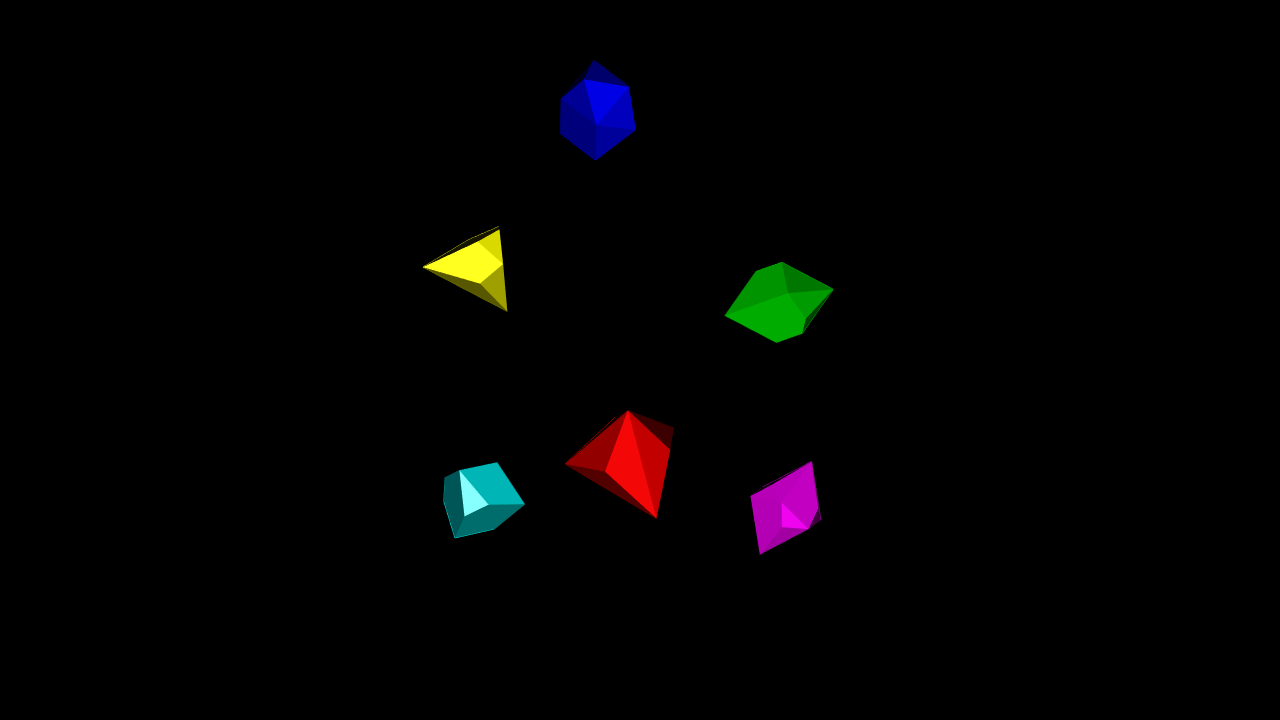
\includegraphics[width=15cm]{images/rpolyhedra_ic18_workshop.png}
 \end{center}
\caption{5 non commonly cited polyhedra from Rpolyhedra database}
\begin{enumerate}
\item \href{https://qbotics.shinyapps.io/rpolyhedra-explorer/?%20_inputs_&polyhedron_color=%22%23FF0000FF%22&polyhedron_name=%22Triakis%20Tetrahedron%22&polyhedron_source=%22dmccooey%22&show_axes=false
}{Triakis Tetrahedron}

\item \href{https://qbotics.shinyapps.io/rpolyhedra-explorer/?_inputs_&polyhedron_color=%22%23FFFF00FF%22&polyhedron_name=%22Self-Dual%20Decahedron%20%2313%20%28canonical%29%22&polyhedron_source=%22dmccooey%22&show_axes=false
}{Self-Dual Decahedron \#13 (canonical)}
\item \href{https://qbotics.shinyapps.io/rpolyhedra-explorer/?_inputs_&polyhedron_color=%22%2300FF00FF%22&polyhedron_name=%22Simplest%20Canonical%20Polyhedron%20with%20Ci%20%3D%20S2%20Symmetry%22&polyhedron_source=%22dmccooey%22&show_axes=false
}{Simplest Canonical Polyhedron with Ci = S2 Symmetry}




\item \href{
https://qbotics.shinyapps.io/rpolyhedra-explorer/?_inputs_&polyhedron_color=%22%2300FFFFFF%22&polyhedron_name=%22Simplest%20Canonical%20Polyhedron%20with%20C3%20Symmetry%20%282%20of%205%29%22&polyhedron_source=%22dmccooey%22&show_axes=false
}{Simplest Canonical Polyhedron with C3 Symmetry 2 of 5}
\item \href{
https://qbotics.shinyapps.io/rpolyhedra-explorer/?_inputs_&polyhedron_color=%22%230000FFFF%22&polyhedron_name=%22augmented%20sphenocorona%20%28J87%29%22&polyhedron_source=%22netlib%22&show_axes=false}{augmented sphenocorona (J87)}
\item \href{
https://qbotics.shinyapps.io/rpolyhedra-explorer/?_inputs_&polyhedron_color=%22%23FF00FFFF%22&polyhedron_name=%22Simplest%20Canonical%20Polyhedron%20with%20S6%20Symmetry%20%281%20of%202%29%22&polyhedron_source=%22dmccooey%22&show_axes=false
}{Simplest Canonical Polyhedron with S6 Symmetry (1 of 2)}
\end{enumerate}
\end{figure}






As part of a project aimed to simplify the access to an open design framework based on polyhedra and tesselations, we needed to retrieve internet information about polyhedra definitions. The work involved the transformation of the data in each source format to a common representation (which can lead to a standard proposal for data exchange) which constitutes a polyhedra database.  

With that in mind, we created a standards based R package, which is available on the CRAN Repository as "Rpolyhedra" and enables users to handle and explore +800 polyhedra definitions with minimum effort. The publication iniciative includes a web explorer \cite{RPOLY_EXPLORER} to lower the burden for non-technical users.


The IC18 talk will focus on the unlocking possibilites derived from the availability of polyhedra constructive methods based on 3D printing and other DIY-technologies for the whole Rpolyhedra database. The participants of the talk will be able to construct from the models available for their exhibits, providing educational resources as well. And we hope, to imagine, design and share different constructive methods to improve the experience about polyhedra out of the screen and the notebook, into the world, playing with the hands.

Polyhedra world is quite rich and we found that when the word polyhedron is mentioned, usually refers to no more than 10 objects (regular solids+ some more polyhedra). With Rpolyhedra, users will be able to research on whole families of polyhedra without the need to master the technical details.

The talk will cover some basic notions about polyhedra and classifications. But will focus on the process of building the database, more a data science project than a mathematical research. Although we found out that some of the most interesting and open source alternatives were not maintained, we migrated, started a curation process and make publicly available the contents to allow new approaches and developments.

The sources currently available are Netlib's Polyhedra\cite{NETLIB}, by Andrew Hume and Visual Polyhedra\cite{DMCCOOEY} by David McCooey. Other databases where found but didn't provide new information (\cite{NAT_ALISON}, \cite{GEORGE_HART}, \cite{WOLFRAM_ALPHA_TETRA},\cite{WIKIPEDIA_TETRA}). One special case is polymake\cite{POLYMAKE}, a language for research in polyhedral geometry, a deep technical research tool which includes database capabilities. 


Along with the creation of the library, the talk will continue with our experiences with existing constructive methods and taking its lessons to the next level showing our experience on Augmented Reality (AR) for interactive polyhedra design. 





\bibliographystyle{plain}

\begin{thebibliography}{10}
\bibitem{NETLIB}{Polyhedra. HUME, Andrew and others. \url{http://www.netlib.org/polyhedra/}}
\bibitem{DMCCOOEY}{Visual Polyhedra, MCCOOEY, David, \url{http://dmccooey.com/polyhedra/}}
\bibitem{RPOLY_EXPLORER}{Polyhedra Explorer, BARANEK, Alejandro and BELEN, Leonardo, \url{https://qbotics.shinyapps.io/rpolyhedra-explorer/}}
\bibitem{NAT_ALISON}{Nat Alison’s polyhedra.js, https://\url{polyhedra.tessera.li/}}
\bibitem{GEORGE_HART}{George Hart Netlib database  republish \url{http://www.georgehart.com/virtual-polyhedra/netlib-info.html}}
\bibitem{WOLFRAM_ALPHA_TETRA}{Wolfram Alpha tetrahedron definition, \url{http://www.wolframalpha.com/input/?i=tetrahedron}}
\bibitem{WIKIPEDIA_TETRA}{Wikipedia tetrahedron definition, \url{https://en.wikipedia.org/wiki/Tetrahedron}}
\bibitem{POLYMAKE}{polymake, \url{https://polymake.org/doku.php}}

\end{thebibliography}



%\section{How to name and upload of this document (CUT AWAY!) } 

%\textit{please delete this section before you submit your proposal}

%\paragraph{Document name} To make it easier for us to store, find and use your proposal, please stick to the following rules:

%\begin{itemize}
% \item Please call the document as \textit{ic18\textunderscore talk\textunderscore YourSurname.pdf}.
% \item Please use no spaces within the document name
%\end{itemize}

%\paragraph{Submit your proposal}

%To submit your proposal, send the documentation to ic18@imaginary.org
%with the text ``Talk Submission''  in the subject. Please copy your title
%and abstract into the body of the email and attach your complete
%proposal as one pdf document. 


%\paragraph{Submission deadline}
%The deadline for proposal submission is
%August 15th, 2018. We strongly encourage you to submit your proposal as
%early as possible (though the decision of the scientific committee does
%not depend on your submission date).  



\end{document}          
